% Options for packages loaded elsewhere
\PassOptionsToPackage{unicode}{hyperref}
\PassOptionsToPackage{hyphens}{url}
%
\documentclass[
  ignorenonframetext,
]{beamer}
\usepackage{pgfpages}
\setbeamertemplate{caption}[numbered]
\setbeamertemplate{caption label separator}{: }
\setbeamercolor{caption name}{fg=normal text.fg}
\beamertemplatenavigationsymbolsempty
% Prevent slide breaks in the middle of a paragraph
\widowpenalties 1 10000
\raggedbottom
\setbeamertemplate{part page}{
  \centering
  \begin{beamercolorbox}[sep=16pt,center]{part title}
    \usebeamerfont{part title}\insertpart\par
  \end{beamercolorbox}
}
\setbeamertemplate{section page}{
  \centering
  \begin{beamercolorbox}[sep=12pt,center]{part title}
    \usebeamerfont{section title}\insertsection\par
  \end{beamercolorbox}
}
\setbeamertemplate{subsection page}{
  \centering
  \begin{beamercolorbox}[sep=8pt,center]{part title}
    \usebeamerfont{subsection title}\insertsubsection\par
  \end{beamercolorbox}
}
\AtBeginPart{
  \frame{\partpage}
}
\AtBeginSection{
  \ifbibliography
  \else
    \frame{\sectionpage}
  \fi
}
\AtBeginSubsection{
  \frame{\subsectionpage}
}
\usepackage{amsmath,amssymb}
\usepackage{lmodern}
\usepackage{iftex}
\ifPDFTeX
  \usepackage[T1]{fontenc}
  \usepackage[utf8]{inputenc}
  \usepackage{textcomp} % provide euro and other symbols
\else % if luatex or xetex
  \usepackage{unicode-math}
  \defaultfontfeatures{Scale=MatchLowercase}
  \defaultfontfeatures[\rmfamily]{Ligatures=TeX,Scale=1}
\fi
\usecolortheme{beaver}
% Use upquote if available, for straight quotes in verbatim environments
\IfFileExists{upquote.sty}{\usepackage{upquote}}{}
\IfFileExists{microtype.sty}{% use microtype if available
  \usepackage[]{microtype}
  \UseMicrotypeSet[protrusion]{basicmath} % disable protrusion for tt fonts
}{}
\makeatletter
\@ifundefined{KOMAClassName}{% if non-KOMA class
  \IfFileExists{parskip.sty}{%
    \usepackage{parskip}
  }{% else
    \setlength{\parindent}{0pt}
    \setlength{\parskip}{6pt plus 2pt minus 1pt}}
}{% if KOMA class
  \KOMAoptions{parskip=half}}
\makeatother
\usepackage{xcolor}
\IfFileExists{xurl.sty}{\usepackage{xurl}}{} % add URL line breaks if available
\IfFileExists{bookmark.sty}{\usepackage{bookmark}}{\usepackage{hyperref}}
\hypersetup{
  hidelinks,
  pdfcreator={LaTeX via pandoc}}
\urlstyle{same} % disable monospaced font for URLs
\newif\ifbibliography
\setlength{\emergencystretch}{3em} % prevent overfull lines
\providecommand{\tightlist}{%
  \setlength{\itemsep}{0pt}\setlength{\parskip}{0pt}}
\setcounter{secnumdepth}{-\maxdimen} % remove section numbering
\iffalse
https://tex.stackexchange.com/questions/392324/how-to-exclude-total-slide-number-from-beamer-slide
\fi
\setbeamertemplate{navigation symbols}{} 
\setbeamertemplate{footline}{\quad\hfill\insertframenumber\strut\quad}
\usefonttheme[onlymath]{serif}
\setbeamertemplate{itemize items}[circle]
\author[John Koo]{John Koo}
\usepackage{setspace}
\usepackage{float}
\usepackage{mathtools}
\usepackage{natbib}
\usepackage[linesnumbered,ruled,vlined]{algorithm2e}
\setcitestyle{numbers,square,comma}
\usepackage{verbatim}
\usepackage{amsthm}
\usepackage{comment}
\usepackage{graphicx}
\setbeamertemplate{itemize items}[circle]
\ifLuaTeX
  \usepackage{selnolig}  % disable illegal ligatures
\fi

\author{}
\date{\vspace{-2.5em}}

\begin{document}

\begin{frame}[plain]{}
\protect\hypertarget{section}{}
\center

\LARGE

\textcolor{darkred}{Popularity Adjusted Block Models are Generalized Random Dot Product Graphs}

\normalsize

JSM Speed Presentation

August 2022

\begin{columns}[T]
\begin{column}{0.33\textwidth}
\begin{center}\includegraphics[width=67px]{john-koo} \end{center}

John Koo,\\
PhD Student in Statistical Science,\\
Indiana University
\end{column}

\begin{column}{0.33\textwidth}
\begin{center}\includegraphics[width=67px]{minh-tang} \end{center}

Minh Tang,\\
Assistant Professor of Statistics,\\
NC State University
\end{column}

\begin{column}{0.33\textwidth}
\begin{center}\includegraphics[width=67px]{michael-trosset} \end{center}

Michael Trosset,\\
Professor of Statistics,\\
Indiana University
\end{column}
\end{columns}
\end{frame}

\begin{frame}{Community Detection for Networks}
\protect\hypertarget{community-detection-for-networks}{}
\newcommand{\diag}{\text{diag}}
\newcommand{\tr}{\text{Tr}}
\newcommand{\blockdiag}{\text{blockdiag}}
\newcommand{\indep}{\stackrel{\text{ind}}{\sim}}
\newcommand{\iid}{\stackrel{\text{iid}}{\sim}}
\newcommand{\Bernoulli}{\text{Bernoulli}}
\newcommand{\Betadist}{\text{Beta}}
\newcommand{\BG}{\text{BernoulliGraph}}
\newcommand{\Cat}{\text{Categorical}}
\newcommand{\Uniform}{\text{Uniform}}
\newcommand{\RDPG}{\text{RDPG}}
\newcommand{\GRDPG}{\text{GRDPG}}
\newcommand{\PABM}{\text{PABM}}

\begin{center}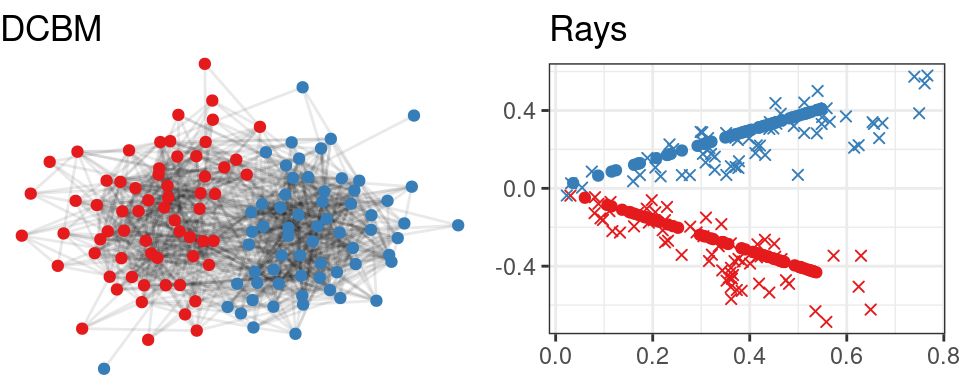
\includegraphics[width=0.5\linewidth]{slides_files/figure-beamer/unnamed-chunk-4-1} \end{center}

\textbf{Def} Popularity Adjusted Block Model (Sengupta and Chen, 2017):

Let each vertex \(i \in [n]\) have \(K\) popularity parameters
\(\lambda_{i1}, ..., \lambda_{iK} \in [0, 1]\).\\
Then \(A \sim \text{BernoulliGraph}(P)\) is a PABM if each
\(P_{ij} = \lambda_{i z_j} \lambda_{j z_i}\)
\end{frame}

\begin{frame}{Popularity Adjusted Block Model}
\protect\hypertarget{popularity-adjusted-block-model}{}
\textbf{Def} Popularity Adjusted Block Model (Sengupta and Chen, 2017):

Let each vertex \(i \in [n]\) have \(K\) popularity parameters
\(\lambda_{i1}, ..., \lambda_{iK} \in [0, 1]\). Then
\(A \sim \text{PABM}(\{\lambda_{ik}\}_K)\) if each
\(P_{ij} = \lambda_{i z_j} \lambda_{j z_i}\).

\textbf{Def} (Noroozi, Rimal, and Pensky, 2020):

\(A\) is sampled from a PABM if \(P\) can be described as:

\begin{enumerate}
\tightlist
\item
  Let each \(P^{(kl)}\) denote the \(n_k \times n_l\) matrix of edge
  probabilities between communities \(k\) and \(l\).
\item
  Organize popularity parameters as vectors
  \(\lambda^{(kl)} \in \mathbb{R}^{n_k}\) such that
  \(\lambda^{(kl)}_i = \lambda_{k_i l}\) is the popularity parameter of
  the \(i\)\textsuperscript{th} vertex of community \(k\) towards
  community \(l\).
\item
  Each block can be decomposed as
  \(P^{(kl)} = \lambda^{(kl)} (\lambda^{(lk)})^\top\).
\end{enumerate}
\end{frame}

\begin{frame}{Generalized Random Dot Product Graph}
\protect\hypertarget{generalized-random-dot-product-graph}{}
\textbf{Def} Generalized Random Dot Product Graph\\
(Rubin-Delanchy, Cape, Tang, Priebe, 2020)

Let \(I_{p,q} = \text{blockdiag}(I_p, -I_q)\) and suppose that
\(x_1, \ldots, x_n \in \mathbb{R}^{p+q}\) are such that
\(x_i^\top I_{p,q} x_j \in [0,1]\).\\
Then \(A \sim \text{GRDPG}_{p, q}(X)\) iff
\(A \sim \text{BernoulliGraph}(X I_{p,q} X^\top)\), where
\(X = \begin{bmatrix} x_1 & \cdots & x_n \end{bmatrix}^\top\).

Adjacency Spectral Embedding (Sussman et al., 2012) estimates
\(x_1, ..., x_n \in \mathbb{R}^{p+q}\) from \(A\):

\begin{enumerate}
\tightlist
\item
  Let \(\hat{\Lambda}\) be the diagonal matrix that contains the
  absolute values of the \(p\) most positive and the \(q\) most negative
  eigenvalues.
\item
  Let \(\hat{V}\) be the matrix whose columns are the corresponding
  eigenvectors.
\item
  Compute \(\hat{X} = \hat{V} \hat{\Lambda}^{1/2}\).
\end{enumerate}

\textbf{Theorem}:
\(\max\limits_i \|\hat{X}_i - Q_n X_i \| = O_P \Big( \frac{(\log n)^c}{n^{1/2}} \Big)\)
as \(n \to \infty\)
\end{frame}

\begin{frame}{Connecting Block Models to the (G)RDPG Model}
\protect\hypertarget{connecting-block-models-to-the-grdpg-model}{}
\begin{columns}[T]
\begin{column}{0.48\textwidth}
\begin{center}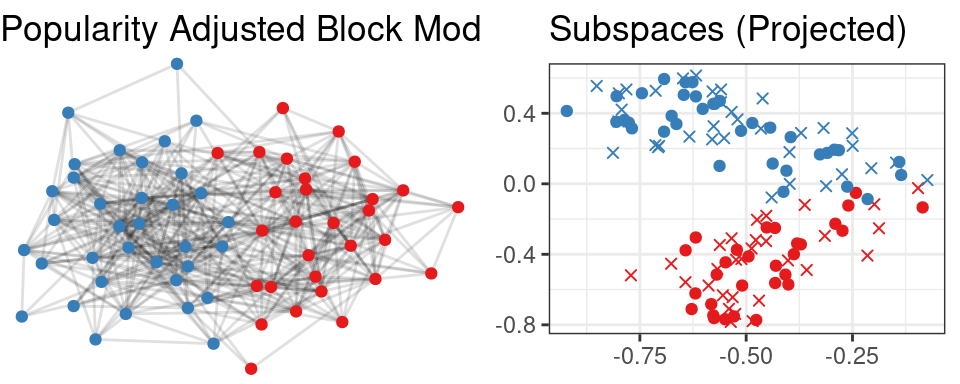
\includegraphics[width=0.5\linewidth]{slides_files/figure-beamer/unnamed-chunk-5-1} \end{center}

\vspace*{.5\baselineskip}

\begin{center}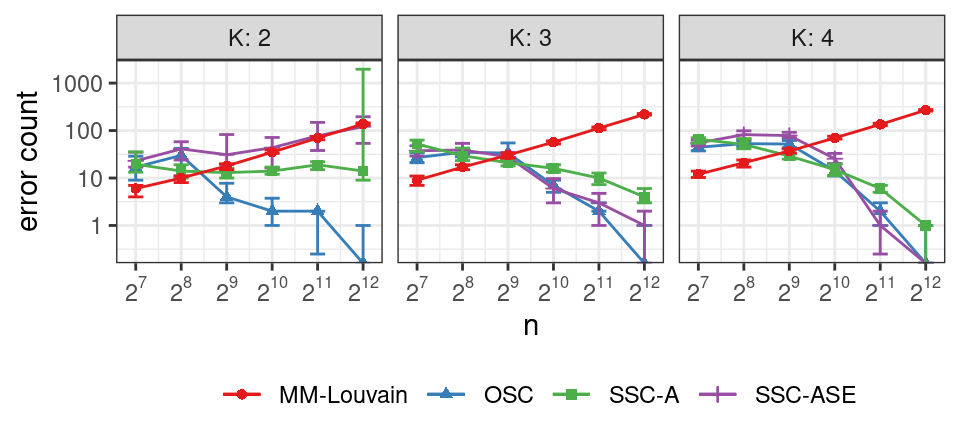
\includegraphics[width=0.5\linewidth]{slides_files/figure-beamer/unnamed-chunk-6-1} \end{center}
\end{column}

\begin{column}{0.48\textwidth}
\vspace*{0\baselineskip}

\begin{center}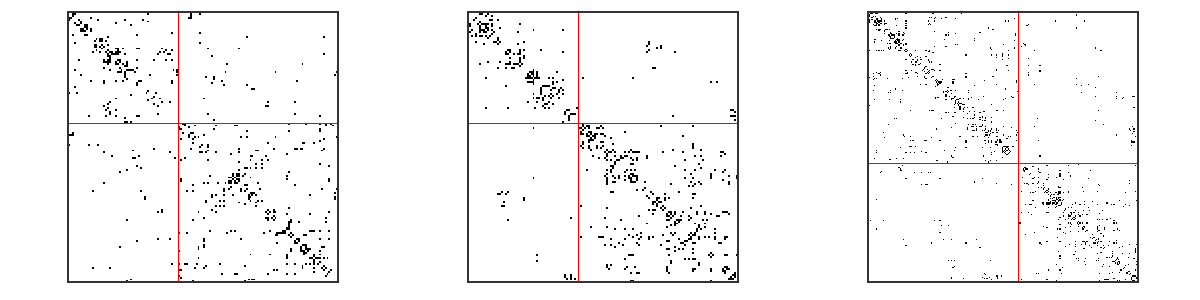
\includegraphics[width=1\linewidth]{slides_files/figure-beamer/unnamed-chunk-7-1} \end{center}
\end{column}
\end{columns}
\end{frame}

\begin{frame}{Connecting the PABM to the GRDPG}
\protect\hypertarget{connecting-the-pabm-to-the-grdpg}{}
\textbf{Theorem} (KTT): \(A \sim \text{PABM}(\{\lambda_{ik}\}_K)\) is
equivalent to \(A \sim \text{GRDPG}_{p, q}(X U)\) with

\begin{itemize}
\tightlist
\item
  \(p = K (K + 1) / 2\), \(q = K (K - 1) / 2\);
\item
  \(U\) is an orthogonal matrix;
\item
  \(X \in \mathbb{R}^{n \times K^2}\) is a block diagonal matrix
  composed of popularity vectors with each block corresponding to a
  community.
\end{itemize}

\[X = \begin{bmatrix}
\Lambda^{(1)} & \cdots & 0 \\
0 & \ddots & 0 \\
0 & \cdots & \Lambda^{(K)}
\end{bmatrix} 
\in \mathbb{R}^{n \times K^2}\]

\[\Lambda^{(k)} = \begin{bmatrix} 
\lambda^{(k1)} & \cdots & \lambda^{(kK)} 
\end{bmatrix} 
\in \mathbb{R}^{n_k \times K}\]

\[A \sim \text{PABM}(\{\lambda_{ik}\}_K) \text{ iff } A \sim \text{GRDPG}_{p, q}(X U)\]
\end{frame}

\begin{frame}{Orthogonal Spectral Clustering}
\protect\hypertarget{orthogonal-spectral-clustering}{}
\textbf{Theorem} (KTT): If \(P = V \Lambda V^\top\) and
\(B = n V V^\top\),\\
then \(B_{ij} = 0\) if \(z_i \neq z_j\).

\textbf{Algorithm}: Orthogonal Spectral Clustering:

\begin{enumerate}
\tightlist
\item
  Let \(V\) be the eigenvectors of \(A\) corresponding to the
  \(K (K+1)/2\) most positive and \(K (K-1) / 2\) most negative
  eigenvalues.
\item
  Compute \(B = |n V V^\top|\) applying \(|\cdot|\) entry-wise.
\item
  Construct graph \(G\) using \(B\) as its similarity matrix.
\item
  Partition \(G\) into \(K\) disconnected subgraphs.
\end{enumerate}

\textbf{Theorem} (KTT): Let \(\hat{B}\) with entries \(\hat{B}_{ij}\) be
the affinity matrix from OSC. Then \(\forall\) pairs \((i, j)\)
belonging to different communities and sparsity factor satisfying
\(n \rho_n = \omega\big((\log n)^{4c}\big)\),\\
\(\max_{i, j} \hat{B}_{ij} = O_P \Big( \frac{(\log n)^c}{\sqrt{n \rho_n}} \Big)\)
as \(n \to \infty\).

\textbf{Corollary}: OSC results in zero clustering error as
\(n \to \infty\), with probability 1.
\end{frame}

\begin{frame}{Simulation Results}
\protect\hypertarget{simulation-results}{}
We compare four algorithms for community detection on randomly generated
PABMs:

\begin{itemize}
\tightlist
\item
  Modularity Maximization (Sengupta and Chen) using the Louvain
  algorithm;
\item
  Orthogonal Spectral Clustering (KTT);
\item
  Sparse Subspace Clustering on the columns of \(A\)\\
  (Noorozi, Rimal, Pensky);
\item
  Sparse Subspace Clustering on the ASE (KTT).
\end{itemize}

\begin{center}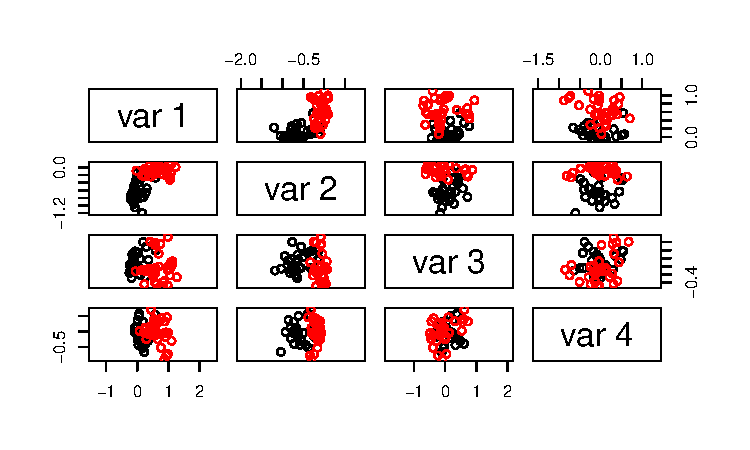
\includegraphics[width=1\linewidth]{slides_files/figure-beamer/unnamed-chunk-8-1} \end{center}
\end{frame}

\begin{frame}{Popularity Adjusted Block Models are Generalized Random
Dot Product Graphs}
\protect\hypertarget{popularity-adjusted-block-models-are-generalized-random-dot-product-graphs}{}
Published in \emph{Journal of Computational and Graphical Statistics}

arXiv preprint: \url{https://arxiv.org/abs/2109.04010}

GitHub repository: \url{https://github.com/johneverettkoo/pabm-grdpg}

R package: \url{https://github.com/johneverettkoo/osc}
\end{frame}

\end{document}
